\documentclass[10pt,a4paper,landscape]{article}
\usepackage[utf8]{inputenc}
\usepackage[T1]{fontenc}
\usepackage{amsmath}
\usepackage{amsfonts}
\usepackage{amssymb}
\usepackage{graphicx}
\usepackage{lscape}
\usepackage{array}
\usepackage[OT1]{fontenc}
\usepackage[utf8]{inputenc}
\usepackage[none]{hyphenat}
\usepackage{fancyhdr}
\usepackage{eso-pic, graphicx}
\usepackage{multirow}
\usepackage{longtable}
\usepackage[left=0.1cm,right=0.1cm,top=2cm,bottom=2cm]{geometry}
\usepackage[french]{babel}

\graphicspath{ {\VAR{image_path}} }
\newcommand\BackgroundPic{
\put(-4,0){
\parbox[b][\paperheight]{\paperwidth}{
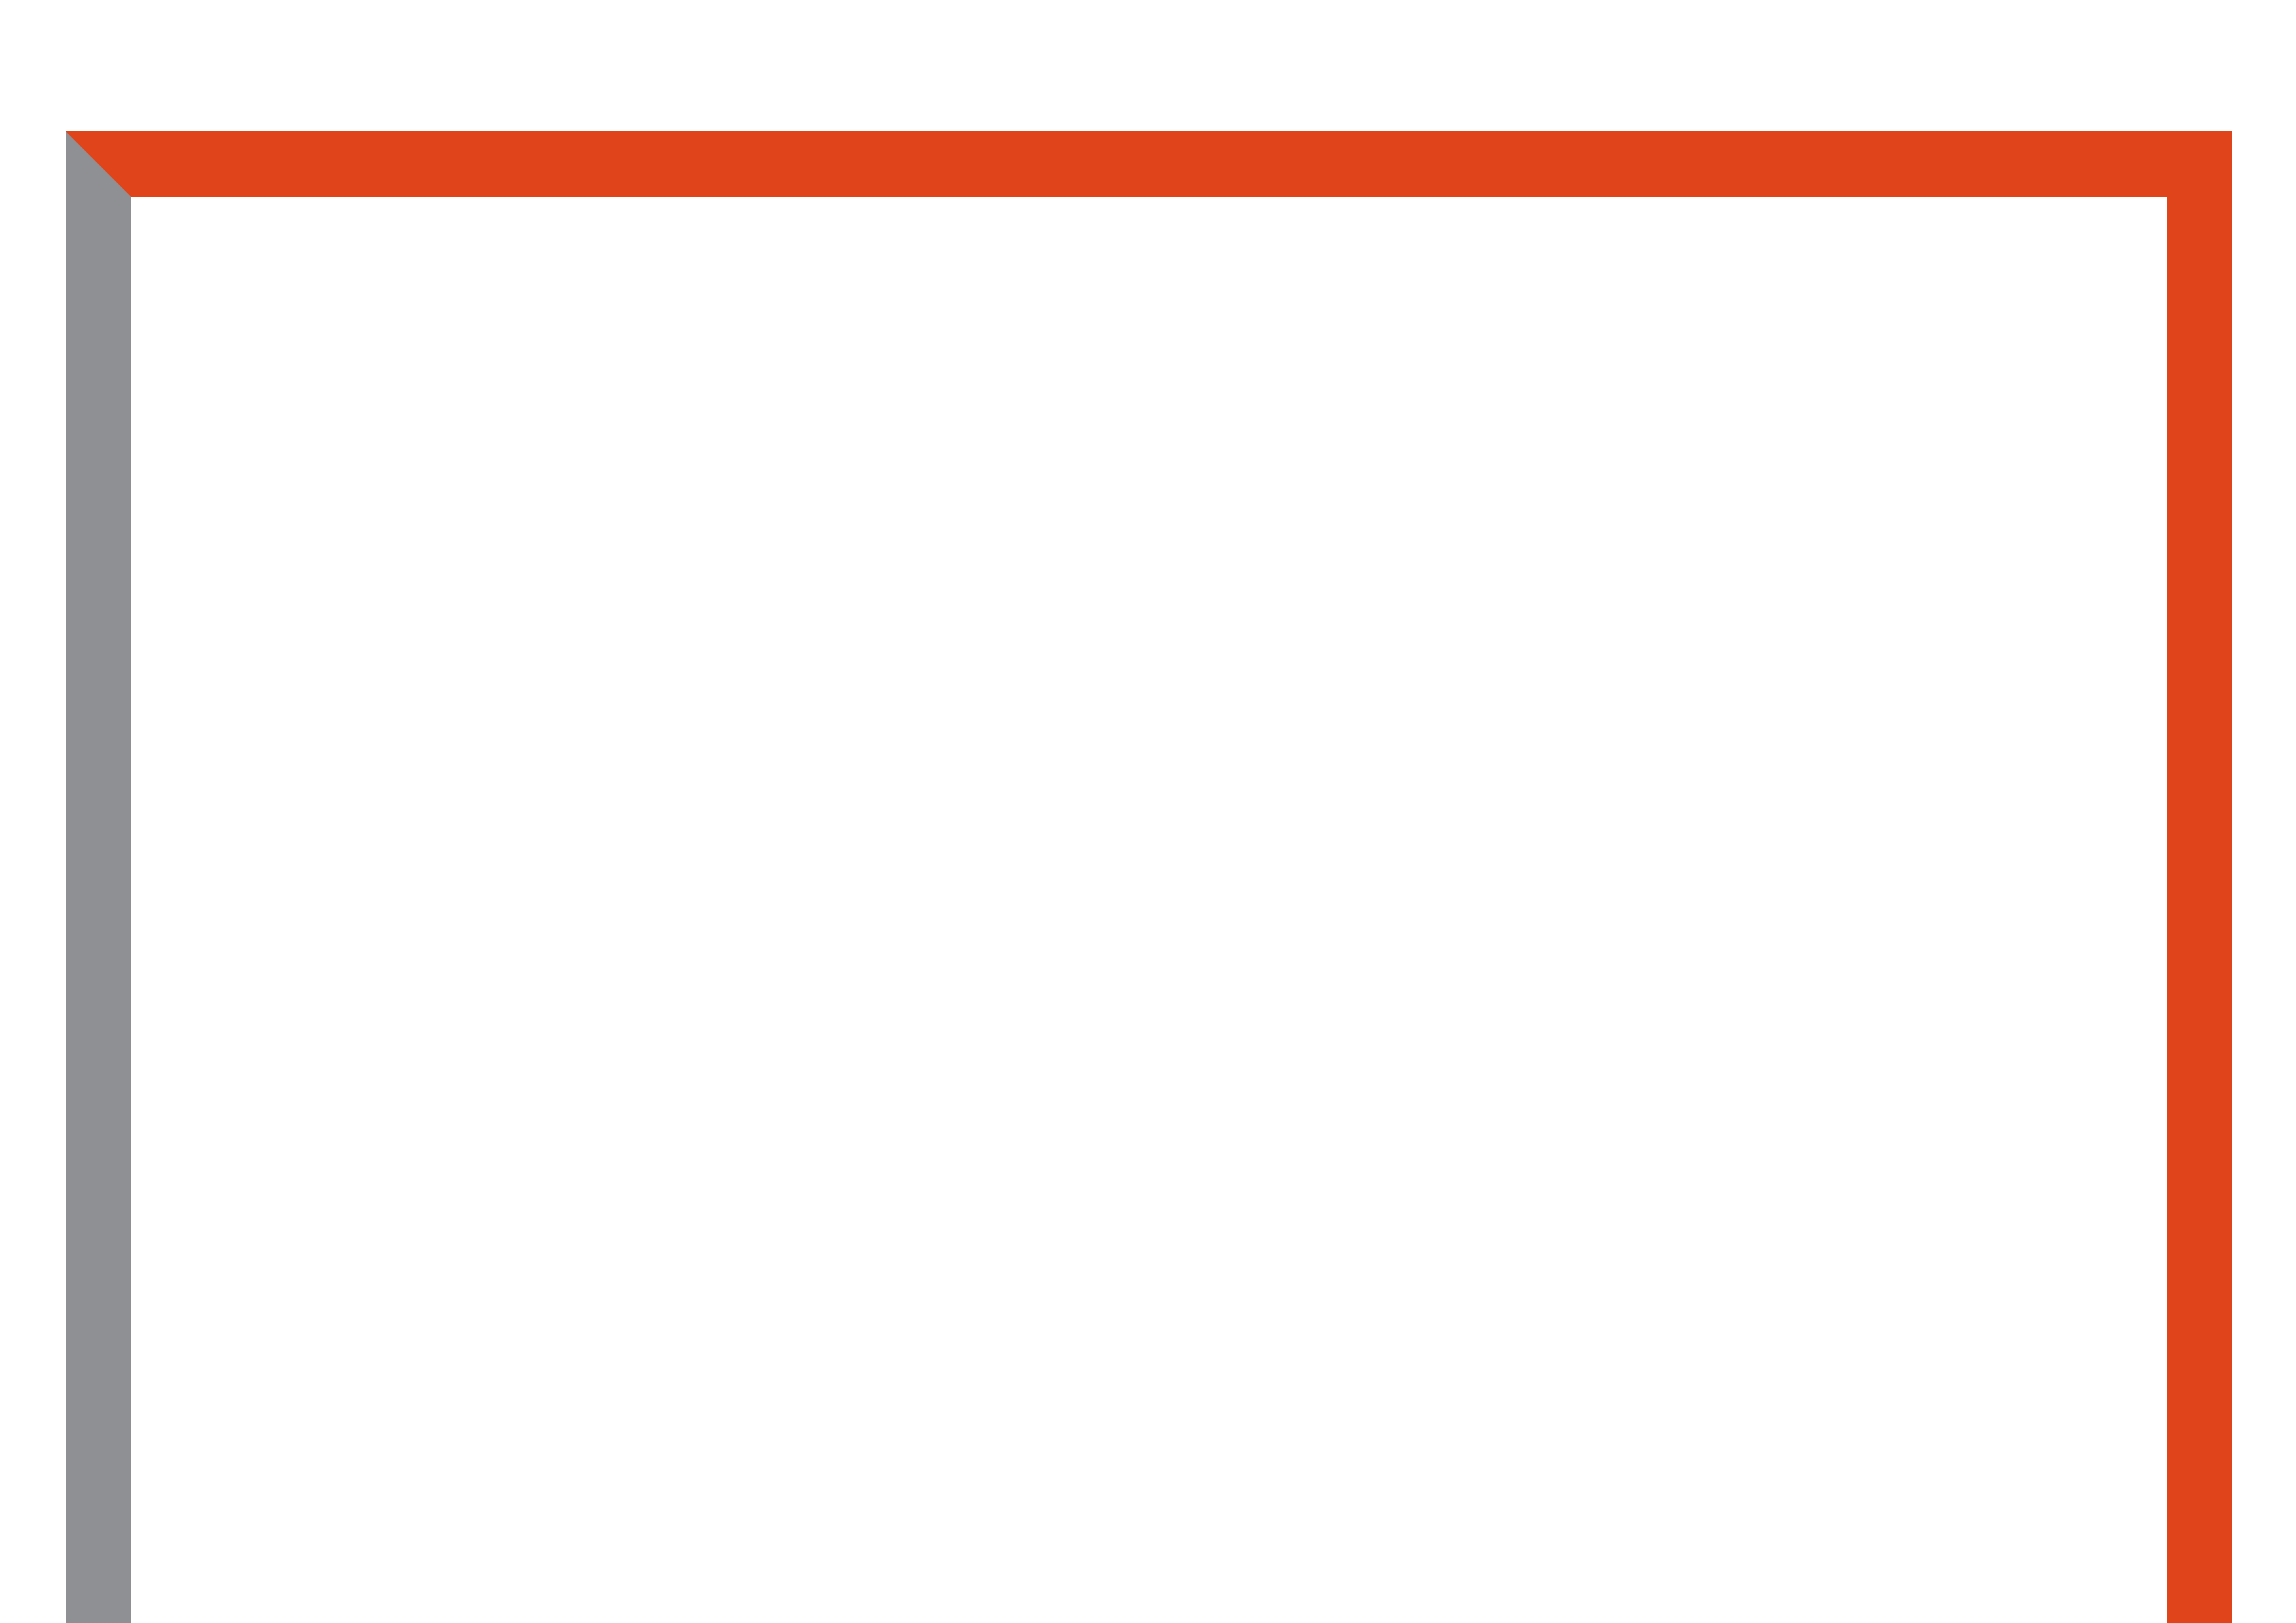
\includegraphics[width=\paperwidth,height=\paperheight]{CharteGraphiquePresentationCorps}
}}}


\begin{document}


\AddToShipoutPicture*{\BackgroundPic}


\begin{center}

\begin{LARGE}
. \vspace{1cm}
\end{LARGE}

\begin{LARGE}
IFNTI : Maquette \VAR{titre}
\end{LARGE}

\begin{longtable}{|c|m{6cm}|m{2.5cm}|m{5cm}|m{1cm}|m{2cm}|m{3cm}|m{3cm}|}
\hline
\centering Semestre & \centering Intitulé UE & \centering Type UE & \centering Matières & \centering Crédit UE & \centering Volume Horaire (H) & \centering Enseignant principal & \centering Enseignant secondaire \arraybackslash  \\ 
\hline
\BLOCK{ for semestre_data in semestres_data }
\BLOCK{ set len_ue = semestre_data.ues|length }
\BLOCK{if len_ue > 0}
\BLOCK{ set nb_total_row = total_row*3 }
\multicolumn{1}{|c|}{\multirow{\VAR{nb_total_row}}{*}{\centering \VAR{semestre_data.semsetre.libelle} }}
	\BLOCK{ for ue in semestre_data.ues }
	\BLOCK{ set nb_row = ue.matiere_set.count() }
	\BLOCK{ set no_row = false if nb_row > 0 else true }
	\BLOCK{ set nb_row = nb_row+6 if nb_row == 0 else nb_row*3+nb_row }
     & \multirow{\VAR{nb_row}}{*}{\parbox{6cm}{\centering \VAR{ue.libelle} \VAR{nb_row}}}
     & \multirow{\VAR{nb_row}}{*}{\parbox{2.5cm}{\centering \VAR{ue.type}}} 
     	& 
     	& \multirow{\VAR{nb_row}}{*}{\parbox{1cm}{\centering \VAR{ue.nbreCredits}}}
     	& & 
     	& \multirow{\VAR{nb_row}}{*}{\parbox{3cm}{\centering \VAR{ue.enseignant}}} \arraybackslash \\ 
    
	\BLOCK{if not no_row}
	\BLOCK{ for matiere in ue.matiere_set.all() }
     & & & \multirow{3}{*}{\parbox{5cm}{\centering \VAR{matiere.libelle} }} 
     		& & \multirow{3}{*}{\parbox{2cm}{\centering \VAR{matiere.heures} }}  
     		& \multirow{3}{*}{\parbox{3cm}{\centering \VAR{matiere.enseignant} }} 
     		& \\
     & & & & & & & \\
     & & & & & & & \\
     & & & & & & & \\
	\BLOCK{ if not loop.last }
	\cline{4-4} \cline{6-7}
	\BLOCK{ endif }
	 \BLOCK{ endfor } 
    
	 \BLOCK{ else }
	 & & & \multirow{3}{*}{\parbox{5cm}{\centering Aucune matiere }} 
     		& & \multirow{3}{*}{\parbox{2cm}{\centering }}  
     		& \multirow{3}{*}{\parbox{3cm}{\centering Aucun prof }} 
     		& \\
     & & & & & & & \\
     & & & & & & & \\
     & & & & & & & \\
	 \BLOCK{ endif }
	 
	 \cline{2-8}
	 \BLOCK{ endfor }     
\BLOCK{ if not loop.last }
\hline
\BLOCK{ endif }
\BLOCK{ endif }
\BLOCK{ endfor }
\hline
\centering Total &  &  &  & \centering \VAR{total_credit} & \centering \VAR{total_horair} &  &  \\ 
\hline 
\end{longtable}

\end{center}



\end{document}
